\documentclass[a4paper,fleqn]{cas-sc}
\usepackage[numbers,sort&compress]{natbib}
\usepackage{needspace}
\usepackage{amsmath,amssymb,booktabs,graphicx,multirow,array,tabularx,placeins,float}
\usepackage{xcolor}
\graphicspath{{figs/}}
\newcolumntype{Y}{>{\raggedright\arraybackslash}X}

\begin{document}
\shorttitle{Global and Token-Level Graph--Text Learning}
\shortauthors{Zang et al.}
\title[mode=title]{Global and Token-Level Crystallographic Text for Crystal Property Prediction: Complementarity and Prediction Averaging}
\author[1]{Huaijuan Zang}\ead{zanghj@hfut.edu.cn}
\author[1]{Yunfan Peng}\cormark[1]
\author[2]{Chong Zhao}\ead{zhaochong@hfut.edu.cn}
\author[1]{Fan Yang}\ead{2021800201@hfut.edu.cn}
\author[3]{Feng Hong}\ead{hongfeng@czu.edu.cn}
\author[1]{Liangfeng Xu}\ead{xulfcjn@hfut.edu.cn}
\affiliation[1]{organization={School of Computer and Information, Hefei University of Technology}, city={Hefei}, country={China}}
\affiliation[2]{organization={Engineering Quality Education Center, Hefei University of Technology}, city={Hefei}, country={China}}
\affiliation[3]{organization={Chizhou University}, city={Chizhou}, country={China}}
\cortext[1]{Corresponding author: Yunfan Peng}

\begin{abstract}
Crystal property prediction can combine periodic crystal graphs with crystallographic text generated from the same structure. In this setting, the graph captures numerical geometry and local connectivity, while the text provides a document-level CLS representation and contextual token representations that expose different structural abstractions. We study graph-conditioned cosine-normalized token attention together with independently trained global and token-level predictors on six JARVIS and four Materials Project tasks. Under fixed splits, two independent runs, and a fixed 0.5/0.5 prediction-level mean, the combined predictor reduces macro MAE by approximately 5.9\% relative to the Global baseline; it improves over Global on all ten tasks in each run and over both constituent predictors on nine of ten tasks in each run. Same-view controls show that ordinary prediction averaging accounts for a substantial fraction of the gain, and the present evidence does not establish superiority over token-only ensembling. Validation-only message-, latent-, and shared-backbone interaction studies show property-dependent behavior and are treated as diagnostic probes rather than as a controlled ranking of fusion locations. The results support sample-aligned prediction complementarity as a reproducible empirical finding under the stated protocol.
\end{abstract}
\begin{keywords}crystal property prediction \sep graph neural network \sep materials language model \sep global text representation \sep token-level representation \sep graph--token attention
\end{keywords}
\maketitle

\section{Introduction}
Computational materials discovery increasingly combines high-throughput electronic-structure calculations with data-driven candidate prioritization, supported by repositories and tooling such as the Materials Project, JARVIS, AFLOW, OQMD, and Matminer \citep{jain2013materialsproject,choudhary2020jarvis,curtarolo2012aflow,saal2013oqmd,ward2018matminer}. Density functional theory provides a principled route to energies, electronic structure, and mechanical response, but repeated calculations over large chemical and structural spaces remain costly. Learned surrogate models can prioritize candidates and provide rapid estimates when their inputs preserve the structural factors that control a target. Crystal structures are naturally represented as periodic graphs: atoms form nodes, local neighbor relations form edges, and geometric features characterize periodic interactions. CGCNN established direct message passing on crystal graphs \citep{xie2018cgcnn}; SchNet introduced continuous-filter convolutions for atomistic coordinates \citep{schutt2018schnet}; MEGNet incorporated edge, node, and global states \citep{chen2019megnet}; ALIGNN explicitly propagated bond-angle information \citep{choudhary2021alignn}; and M3GNet and CHGNet extended expressive atomistic learning toward transferable and pretrained representations \citep{chen2022m3gnet,deng2023chgnet}.

Geometry, however, is not the only compact description of a crystal. A graph records atomic species, neighbor relations, distances, angles, and local environments, but a crystallographic description can explicitly name coordination polyhedra, their connectivity, dimensionality, symmetry, and recurring structural motifs. Such language is derived from the structure and is therefore not an independent experimental modality, yet it reorganizes structural information into chemically meaningful abstractions. The graph and text views overlap in content while differing in representation: the graph is local, numerical, and permutation invariant; the description is sequential, symbolic, and biased toward recognizable concepts. Their partial redundancy makes graph--text learning plausible, whereas their different abstraction levels create an opportunity for complementary errors.

Automated description systems such as Robocrystallographer convert structures into reproducible text \citep{ganose2019robocrystallographer}. Transformer encoders \citep{vaswani2017attention,devlin2019bert} and scientific or materials adaptations such as SciBERT, MatBERT, and MatSciBERT provide contextual representations for specialized terminology \citep{beltagy2019scibert,walker2021matbert,gupta2022matscibert}. Text-only LLM-Prop further demonstrates that structured crystal descriptions can support property prediction \citep{rubungo2025llmprop}. Existing multimodal materials models, including CrysMMNet and LatticeLingo, demonstrate that structural and linguistic signals can be combined \citep{das2023crysmmnet,munjal2024latticelingo}. A common design compresses a complete token sequence into a global document representation and concatenates it with a graph representation. This representation is compact, but tokens naming a coordination number, polyhedron, axis, or space group are no longer individually addressable.

Token-level graph--text interaction offers a direct way to retain fine-grained language information, but naive cross-attention can be numerically misleading. For projected graph query $q$ and token key $k_j$, standard scaled dot-product attention uses $s_j=q^\top k_j/\sqrt d$. The score depends jointly on angular alignment and vector norms. In heterogeneous graph and language spaces, large or unequal norms can produce logits spanning tens or hundreds, causing softmax to behave almost as an argmax. An effective token count close to one can consequently reflect scale-driven saturation rather than precise semantic localization; the present study does not use this diagnostic alone to establish chemical meaning.

The central question is therefore not merely whether text should be used with a graph representation, but where document-level and token-level textual information should interact in graph--text crystal property prediction. In this work, global representation refers specifically to the MatBERT CLS embedding of the tokenized crystallographic description available within the maximum sequence length, whereas token-level representation refers to graph-conditioned aggregation over contextual MatBERT token states. This is distinct from traditional atom-level, subgraph-level, molecule-level, or crystal-level representation hierarchies; the focus here is on different abstraction levels within the same generated crystallographic text.

Several fusion locations are plausible. Message-level interaction injects textual information into graph message passing. Latent-level interaction combines CLS and token features inside one representation. Shared-backbone prediction fusion uses one graph encoder with separate textual heads. Independent prediction-level fusion keeps global and token-level predictors separate and combines their outputs. Latent or message-level fusion can be appealing, but it also introduces a mismatch: the CLS vector summarizes the whole description, whereas token states preserve position-specific contextual evidence. Compressing, gating, or multiplicatively coupling these heterogeneous features can suppress useful token variation, overemphasize broad document context, or make the representation sensitive to property-specific correlations. In the present experiments, interaction signals are often measurable, but direct message-, latent-, and shared-backbone interactions show more property-dependent behavior than independent prediction-level fusion.

We therefore formulate the contribution as an empirical study of fusion location for document-level and token-level textual representations in graph--text crystal property prediction. The final framework keeps a global textual pathway and a token-level textual pathway as independently trained predictors, then studies how their sample-aligned outputs and errors relate. Rather than treating earlier fusion as automatically preferable, we ask whether these two textual abstraction levels are more reliably used through separate predictive pathways and prediction-level complementarity.

Our contributions are fourfold. First, we investigate graph-conditioned, cosine-normalized token extraction from frozen MatBERT contextual states for crystal property prediction. Second, in addition to the main independently trained pathways, we perform a controlled validation ablation that compares CLS pooling, masked contextual-token mean pooling, and graph-conditioned cosine attention under a common prediction head and objective. Third, we analyze prediction complementarity through paired sample-level errors, oracle diagnostics, same-view controls, and fixed cross-view prediction averaging. Fourth, we use validation-only message-level, latent-level, and shared-backbone variants as diagnostic probes of interaction behavior, without claiming a controlled ranking among fusion locations.

\section{Related Work}
\subsection{Crystal graph neural networks}
Crystal GNNs can be organized by the geometric information emphasized in message passing. Distance-based methods use local neighborhoods and radial functions. CGCNN learns edge-conditioned updates from atom and bond descriptors \citep{xie2018cgcnn}, while SchNet learns continuous filters from pair distances \citep{schutt2018schnet}. State-based architectures such as MEGNet jointly update edges, nodes, and global attributes, enabling broad materials and molecular prediction \citep{chen2019megnet}.

Directional models enrich radial descriptions with angular structure. DimeNet constructs directional messages using radial and spherical basis functions \citep{gasteiger2020dimenet}; ALIGNN alternates atomistic and line-graph propagation to model bond angles explicitly \citep{choudhary2021alignn}. Equivariant networks constrain feature transformations under rotations and can achieve high data efficiency for atomistic energies and forces; NequIP is a representative example \citep{batzner2022nequip}. Periodic graph transformers include Matformer and the complete geometric representation of ComFormer \citep{yan2022matformer,yan2024comformer}. SFTGNN introduces spherical-Fourier-enhanced crystal message passing \citep{jiang2025sftgnn}. Composition-only predictors such as Roost and CrabNet provide complementary structure-free references \citep{goodall2020roost,wang2021crabnet}. Related foundation-model efforts in materials increasingly emphasize transferable atomistic or conversational representations, including universal interatomic potentials and multimodal materials assistants \citep{chen2022m3gnet,deng2023chgnet,batatia2023mace,tang2025matterchat}. These approaches primarily solve geometric, atomistic, or compositional representation; they do not by themselves determine how graph information should interact with document-level and token-level crystallographic language representations.

\subsection{Materials language models}
Scientific language differs from general prose through dense entities, formulae, measurement conventions, and domain-specific relations. Materials text additionally contains chemical formulae, space-group symbols, coordination terminology, bonding descriptions, and names for structural prototypes or motifs. MatBERT adapts transformer language modeling to materials corpora, and MatSciBERT provides a domain scientific encoder suited to materials-related extraction and representation \citep{walker2021matbert,gupta2022matscibert}. Their contextual token states offer richer semantics than fixed word vectors, but downstream use often retains only a pooled or CLS representation.

Robocrystallographer provides a controlled interface between structure and language by generating descriptions of symmetry, coordination, and connectivity from a crystal structure \citep{ganose2019robocrystallographer}. This consistency is valuable for multimodal learning: differences in text arise from structural differences rather than uncontrolled author style. Nevertheless, generated descriptions inherit the heuristics and vocabulary of the description engine, so text should be understood as a complementary structural view rather than an independent ground truth.

\subsection{Multimodal materials learning}
Multimodal representation learning has been strongly shaped by image--text alignment models such as CLIP, ALBEF, and BLIP, which show that paired modalities can be connected through contrastive objectives, cross-modal attention, and bootstrapped caption supervision \citep{radford2021clip,li2021albef,li2022blip}. These models motivate a general principle: multimodal learning can benefit from both shared alignment spaces and modality-specific representations. For crystal property prediction, however, the setting differs because the text description is generated from the crystal structure rather than collected as an independent observation. The modalities are therefore partially redundant, and the main question becomes how different abstractions of the same material should be exploited.

Multimodal materials learning has combined structure, composition, images, spectra, and text for prediction or representation learning. Graph--text models are particularly attractive because both modalities can be generated for the same crystal and aligned at the sample level. CrysMMNet combines crystal-graph representations with document-level language representations, whereas LatticeLingo studies descriptions constructed at local, semiglobal, and global structural scopes \citep{das2023crysmmnet,munjal2024latticelingo}. CAST introduces cross-attention-based structure--text interaction, while Hybrid-LLM-GNN combines graph and materials-language embeddings for cross-property prediction \citep{lee2025cast,li2025hybridllmgnn}. CLICS explores graph--text contrastive learning, and MatterChat broadens materials multimodality toward conversational foundation models \citep{ozawa2024clics,tang2025matterchat}. In contrast, the present study focuses on representation granularity within one generated crystallographic description: document-level CLS versus contextual token states, and on their predictive complementarity under a common benchmark protocol.

\subsection{Fine-grained cross-modal attention}
Cross-attention is widely used to align elements of two modalities following scaled dot-product attention in the Transformer \citep{vaswani2017attention}. In materials prediction, a graph-level query and textual token keys provide a natural asymmetric form: the crystal asks which parts of its own description are useful. Dot-product similarity, however, combines direction and norm. When encoders and projections have different scale statistics, attention sharpness can be governed by norms instead of correspondence. Query-Key Normalization motivates normalizing both projections to prevent arbitrary softmax saturation \citep{henry2020qknorm}. Related normalization ideas also appear in contrastive learning, where CLIP uses normalized image and text features with a learned temperature to stabilize alignment \citep{radford2021clip}. Our token pathway adopts a normalized query--key formulation and treats entropy, effective token count, and maximum attention as diagnostics of token selection rather than as direct evidence of chemical causality.

\section{Methodology}
\subsection{Problem formulation}
Let a sample be $(G,T,y)$, where $G=(V,E)$ is a periodic crystal graph, $T=(w_1,\ldots,w_L)$ is the Robocrystallographer description, and $y\in\mathbb{R}$ is a scalar property. The goal is to learn $f(G,T)$ minimizing mean absolute error (MAE). We construct two predictors, $f_g$ and $f_t$, that use the same material input but different textual abstraction levels, and then combine their predictions at the output level.

\subsection{Global and token-level prediction framework}
Figure~\ref{fig:overall} traces the complete data flow without implying a single joint latent-fusion network. Formally, $\hat y_g=f_{\mathrm{Global}}(G,T)$ and $\hat y_t=f_{\mathrm{Token}}(G,T)$ are produced by independently trained models with checkpoints selected on the validation set. Each predictor contains its own SFTGNN instance. The two instances have the same architecture---92-dimensional atom inputs, five SFTConv layers, 128-dimensional node states, and mean pooling---but their parameters are not shared. Their text processing differs by abstraction level: the global pathway reads the MatBERT CLS state of the tokenized description available within the maximum sequence length, whereas the token-level pathway retains eligible non-special contextual token states and applies graph-conditioned attention. The final prediction-level mean is applied only to sample-aligned outputs. The comparison between the individual Global and Token predictors does not isolate textual granularity as a single causal factor, because their prediction heads and training objectives also differ: the Global path uses direct graph--CLS regression, whereas the Token path uses graph-conditioned token aggregation and an auxiliary graph loss.

\begin{figure}[pos=t]\centering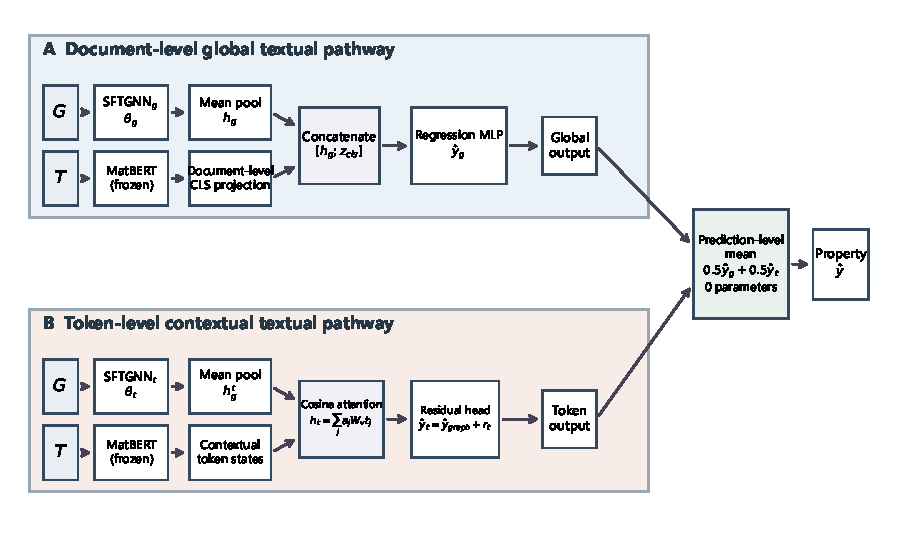
\includegraphics[width=\linewidth]{overall_framework_v9.pdf}
\caption{Global and token-level graph--text learning framework. A global textual pathway uses the document-level MatBERT CLS representation, whereas a token-level pathway uses graph-conditioned cosine attention over contextual token states. The pathways are trained independently under matched graph-encoder architectures, enabling prediction-level complementarity to be evaluated without a shared latent interaction module. Message-, latent-, and shared-backbone interaction variants are analyzed separately as diagnostic studies because their behavior is property dependent.}\label{fig:overall}\end{figure}

\subsection{Spherical-harmonic graph encoder}
For edge $(j,i)$, the implementation computes a radial feature from reciprocal distance, $e^r_{ij}=\mathrm{MLP}_{r}(\mathrm{RBF}(1/d_{ij}))\in\mathbb{R}^{64}$, and projects spherical harmonics to $e^s_{ij}\in\mathbb{R}^{64}$. With $h_i,h_j\in\mathbb{R}^{128}$, the formal SFTConv implementation is
\begin{align}
u_{ij}&=[h_i;h_j;e^r_{ij};e^s_{ij}]\in\mathbb{R}^{384},\\
m_{ij}&=\sigma(\mathrm{MLP}_{gate}([h_i;h_j;e^r_{ij}]))\odot\mathrm{MLP}_{msg}(u_{ij}),\\
h'_i&=\mathrm{SiLU}\!\left(h_i+\mathrm{BN}\left(\sum_{j\in\mathcal{N}(i)}m_{ij}\right)\right).
\end{align}
Both MLPs use a 512-dimensional hidden layer and return 128 features. Five updates are followed by mean scatter pooling.

\begin{figure}[pos=t]\centering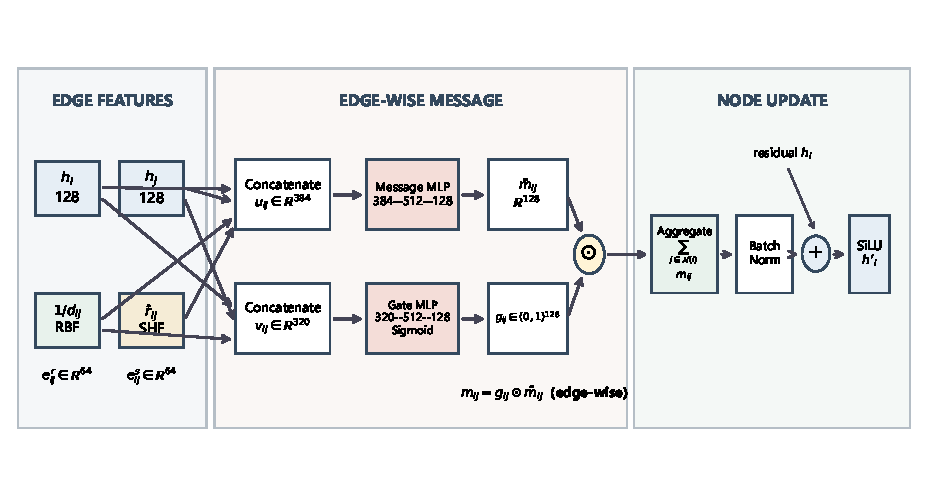
\includegraphics[width=\linewidth]{sftconv_architecture.pdf}
\caption{SFTConv message passing, matching Eq.~(2): the Message MLP output and sigmoid Gate MLP output are multiplied element-wise for each edge before the gated messages are summed over neighbors. Batch normalization, residual addition, and SiLU follow aggregation.}\label{fig:sft}\end{figure}

\subsection{Global textual pathway}
The global pathway corresponds to the original SFTMAT-style baseline used in this study: the SFTGNN graph representation is concatenated directly with the projected MatBERT CLS representation and passed to the regression head.

The CLS state $z_{cls}\in\mathbb{R}^{768}$ is projected by $768\rightarrow128\rightarrow64$ with ReLU. The global pathway concatenates it with the graph representation $h_g$:
\begin{equation}
\hat y_g=\mathrm{MLP}_g([h_g;\phi_{cls}(z_{cls})]).
\end{equation}
This pathway preserves a document-level semantic summary.

\subsection{Token-level textual pathway}
MatBERT is frozen and cached at maximum length 128. The cache stores last hidden states with shape $[N,128,768]$, input IDs, and attention masks in BF16. Padding, CLS, and SEP positions are excluded from normalized attention. Retaining token identity allows graph-conditioned selection while keeping language-model computation outside the training loop.

\subsection{Norm-induced attention collapse}
Raw attention uses $q=W_qh_g$ and $k_j=W_kt_j$. Because $q^\top k_j=\|q\|\|k_j\|\cos\theta_j$, scale and alignment are inseparable. Large norms amplify small angular differences and can make softmax nearly one-hot. We quantify sharpness by entropy $H(a)=-\sum_j a_j\log a_j$ and effective token count $N_{eff}=\exp(H(a))$.

\subsection{Normalized graph-conditioned token attention}
We normalize projected queries and keys and divide cosine similarity by a fixed temperature:
\begin{align}
\bar q&=\frac{W_qh_g}{\|W_qh_g\|_2},\quad
\bar k_j=\frac{W_kt_j}{\|W_kt_j\|_2},\\
a_j&=\frac{\exp(\bar q^\top\bar k_j/\tau)}{\sum_{m\in\mathcal M}\exp(\bar q^\top\bar k_m/\tau)},\quad \tau=0.5,\\
h_t&=\mathrm{LayerNorm}\left(\sum_{j\in\mathcal M}a_jW_vt_j\right)\in\mathbb{R}^{128}.
\end{align}
$\mathcal M$ contains valid non-special tokens.

\begin{figure}[pos=t]\centering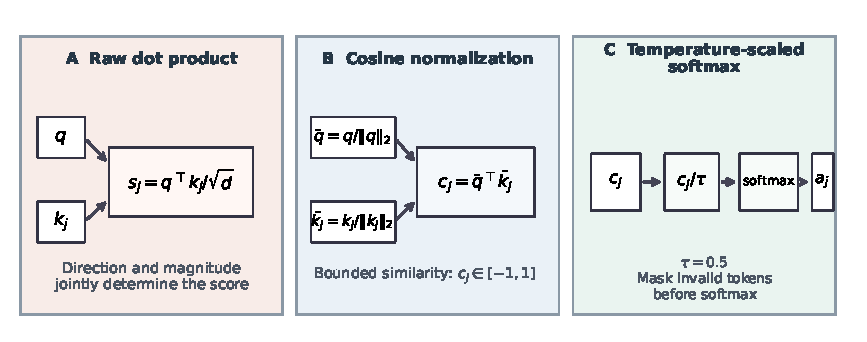
\includegraphics[width=\linewidth]{attention_temperature.pdf}
\caption{Mechanism of graph-conditioned token attention. Raw dot products combine vector direction and magnitude, cosine normalization bounds the similarity, and temperature-scaled softmax converts normalized scores into masked attention weights. The diagram contains no measured attention values.}\label{fig:attention}\end{figure}

\subsection{Token-level predictor}
The token-level predictor first produces a graph-only estimate and then a text-conditioned correction:
\begin{equation}
\hat y_{graph}=\psi_g(h_g),\qquad r_t=\psi_r([h_g;h_t]),\qquad \hat y_t=\hat y_{graph}+r_t.
\end{equation}
Both heads use 128 or 256 hidden features with SiLU. Residual prediction is useful because the graph path provides structure-based prediction, while token-level text adjusts samples whose descriptive semantics are informative.

\subsection{Prediction-level combination}
After independent training and checkpoint selection on the validation set, the sample-aligned predictions are combined as
\begin{equation}\label{eq:dual}
\hat y_D=0.5\hat y_g+0.5\hat y_t.
\end{equation}
No validation labels choose the coefficient, and the same rule is used for all ten tasks. Rather than forcing document-level and token-level representations into a shared latent space, this step preserves their individual predictive pathways and exploits complementary prediction errors.

\subsection{Training objective and computational complexity}
The global textual pathway minimizes $\mathcal L_g=|\hat y_g-y|$. The token-level pathway uses $\mathcal L_t=|\hat y_t-y|+0.2|\hat y_{graph}-y|$. Each pathway is trained independently, and its checkpoint is selected by minimum validation MAE. Token attention costs $O(BLd_a)$ beyond graph encoding, with $L=128$ and $d_a=128$. The combined prediction evaluates both predictors, trading additional latency and parameters for improved predictive accuracy.

\FloatBarrier
\section{Experiments}
\subsection{Datasets and tasks}
We evaluate six JARVIS and four Materials Project property-prediction tasks following the benchmark data preparation and fixed partitions adopted by CrysMMNet \citep{das2023crysmmnet}. The underlying crystal structures and property targets originate from JARVIS and the Materials Project \citep{choudhary2020jarvis,jain2013materialsproject}; Matbench provides broader context for standardized materials benchmarks \citep{dunn2020matbench}. The ten tasks cover electronic, energetic, and mechanical properties. For Materials Project bulk and shear moduli, the benchmark loader applies a $\log_{10}$ transformation to the raw GPa targets before training and evaluation; the corresponding MAEs are therefore reported in the transformed target space.

\subsection{Text generation and caching}
Each crystal is converted to a Robocrystallographer description and tokenized by MatBERT. We refer to the tokenized crystallographic description available within the maximum sequence length, rather than assuming that every generated description is fully retained. Sequences use maximum length 128 with truncation and padding masks. The global path reads position zero as the CLS representation; the token path reads the full last-hidden-state tensor and removes CLS, SEP, and PAD from attention eligibility. MatBERT representations are precomputed in BF16 and paired with input IDs and masks, so language-model forward computation is not repeated during property-model training or inference when the cache is available.

\subsection{Training protocol}
The main Global, Token, and Global+Token experiments were repeated with two independent model-training seeds (42 and 43), while all models used the same fixed data partitions. Architecture, hyperparameters, target transformation, MatBERT sequence length, temperature $\tau=0.5$, checkpoint criterion, fixed 0.5/0.5 prediction-level mean, and test protocol were unchanged. For each run, the global textual and token-level textual predictors are initialized and trained independently with batch size 32, evaluation batch size 64, AdamW \citep{loshchilov2019adamw}, learning rate and maximum OneCycleLR rate $10^{-3}$, weight decay $10^{-4}$, BF16 autocast, and a 300-epoch budget. Each predictor is selected by its minimum validation MAE, after which the test set is evaluated once. Predictions are aligned by sample ID and their targets are matched within floating-point precision before averaging; band-gap outputs are clipped to nonnegative values. The interaction-location studies were validation-only diagnostic experiments and used the task and run coverage reported in Section~5.5; they were not uniformly repeated under the two-run main-test protocol.
To isolate textual representation from pathway-specific prediction heads and training objectives, we additionally performed a single-seed matched validation ablation on a balanced six-task subset spanning JARVIS and Materials Project electronic, energetic, and mechanical properties. The CLS, masked-mean, and cosine-attention variants used the same graph encoder, 128-dimensional text output, regression head, MAE objective, optimizer, scheduler, training budget, validation partition, and training seed (42), and differed only in how the MatBERT representation was aggregated. These results were used only for representation-level analysis and were not evaluated on the test set.

\subsection{Evaluation}
MAE is the principal metric because it is in the benchmark target space and limits the influence of extreme errors. Relative gain against the global textual pathway is $(\mathrm{MAE}_g-\mathrm{MAE}_{dual})/\mathrm{MAE}_g\times100\%$. We also report absolute-error Pearson correlation, oracle MAE, and per-sample win fractions on the validation set. Model selection and the fixed 0.5/0.5 rule use the validation set only; the test set is excluded from training, tuning, and checkpoint selection.

The two-run validation predictions further define same-view controls. Let $G_1,G_2$ denote the Global predictions and $T_1,T_2$ the Token predictions from seeds 42 and 43. We compute $GG=(G_1+G_2)/2$ and $TT=(T_1+T_2)/2$, and compare them with the run-matched global--token means $GT_1=(G_1+T_1)/2$ and $GT_2=(G_2+T_2)/2$. All four files for each task contain identical sample-ID sets and ordering; targets agree within a maximum absolute numerical difference of $2.39\times10^{-7}$. No prediction weight is fitted from validation labels.

\FloatBarrier
\section{Results}
\subsection{Overall performance}
\begin{table}[!htbp]\caption{Test-set MAE averaged over two independent runs and relative gain over Global. Values are reported as mean $\pm$ sample standard deviation; lower MAE is better. Bold indicates the best result and underlining indicates the second-best result under the same evaluation protocol. Ranking compares the mean MAE; the standard deviation is displayed as part of the same result.}\label{tab:test}\centering\scriptsize
\resizebox{\linewidth}{!}{\begin{tabular}{lrrrr}\toprule Task&Global&Token&Global+Token&Gain (\%)\\\midrule
JARVIS-MBJ&\underline{0.259641 $\pm$ 0.002825}&0.267325 $\pm$ 0.009433&\textbf{0.251800 $\pm$ 0.001808}&3.011 $\pm$ 1.752\\
JARVIS-OPT&0.124654 $\pm$ 0.003559&\underline{0.119036 $\pm$ 0.004411}&\textbf{0.115764 $\pm$ 0.000876}&7.104 $\pm$ 1.950\\
JARVIS-Formation&0.029453 $\pm$ 0.000692&\underline{0.028832 $\pm$ 0.000190}&\textbf{0.027437 $\pm$ 0.000406}&6.836 $\pm$ 0.810\\
JARVIS-Total&0.032296 $\pm$ 0.000405&\underline{0.031422 $\pm$ 0.000010}&\textbf{0.029796 $\pm$ 0.000167}&7.736 $\pm$ 0.639\\
JARVIS-Bulk&9.60549 $\pm$ 0.14011&\underline{9.40847 $\pm$ 0.09234}&\textbf{9.14175 $\pm$ 0.04797}&4.821 $\pm$ 0.889\\
JARVIS-Shear&8.96774 $\pm$ 0.03243&\underline{8.72852 $\pm$ 0.12811}&\textbf{8.52204 $\pm$ 0.13611}&4.972 $\pm$ 1.174\\
MP-Bandgap&0.211599 $\pm$ 0.003322&\textbf{0.196220 $\pm$ 0.002127}&\underline{0.196354 $\pm$ 0.002946}&7.204 $\pm$ 0.065\\
MP-Formation&0.024373 $\pm$ 0.000796&\underline{0.024256 $\pm$ 0.000511}&\textbf{0.022769 $\pm$ 0.000646}&6.576 $\pm$ 0.399\\
MP-Bulk&0.037610 $\pm$ 0.001028&\underline{0.036156 $\pm$ 0.000402}&\textbf{0.034938 $\pm$ 0.000623}&7.092 $\pm$ 0.884\\
MP-Shear&0.071981 $\pm$ 0.000318&\underline{0.071636 $\pm$ 0.000668}&\textbf{0.069533 $\pm$ 0.000013}&3.400 $\pm$ 0.445\\\midrule
Macro gain&&&&5.875 $\pm$ 0.036\\\bottomrule\end{tabular}}\end{table}

Table~\ref{tab:test} reports test-set MAE as the mean and sample standard deviation over two independent runs. Across the ten tasks, the test partition contributes 24,671 sample-task evaluations per run; this is not a count of unique crystals. The global--token prediction-level combination improves upon the global pathway on all ten tasks in both runs, with an average macro relative MAE reduction of approximately $5.9\%$ (mean $\pm$ sample standard deviation over two independent runs: $5.875\pm0.036\%$). We use this small standard deviation only as evidence of consistency between the two runs, not as a formal significance estimate. In each run, the combined prediction also outperforms both individual pathways on nine of the ten tasks. One task per run is predicted slightly more accurately by the token-level pathway, while the combined prediction remains more accurate than the corresponding global pathway. The average macro relative gains over the global pathway are $5.747\pm0.069\%$ on JARVIS and $6.068\pm0.193\%$ on Materials Project.

The run-wise macro relative MAE reductions are 5.850\% and 5.901\%, showing close agreement in the overall benefit. Based on the task-wise means over the two runs, the combined prediction reduces MAE by 3.011--7.204\% for electronic properties, 6.576--7.736\% for energetic properties, and 3.400--7.092\% for mechanical properties.

\subsection{Comparison with existing methods}
\begin{table}[pos=H]
\caption{Reference comparison under different protocols on JARVIS. MAE units are eV/atom for formation and total energy, eV for band gaps, and GPa for elastic moduli. Published values follow the evaluation protocol of each study; dashes indicate unreported properties. Bold values mark the lowest reported MAE and underlined values the second-lowest reported MAE in each property column for visual reference only. Because data partitions, target transformations, and test protocols differ across studies, these marks do not constitute a protocol-matched cross-study ranking.}
\label{tab:jarvis_lit}\centering\scriptsize
\resizebox{\linewidth}{!}{\begin{tabular}{lrrrrrr}\toprule
Method&Formation energy&Bandgap OPT&Bandgap MBJ&Total energy&Bulk $K_v$&Shear $G_v$\\\midrule
CGCNN&0.063&0.200&0.413&0.078&14.47&11.75\\
SchNet&0.045&0.192&0.433&0.047&14.33&10.67\\
MEGNet&0.047&0.145&0.344&0.058&15.11&13.09\\
GATGNN&0.047&0.170&0.513&0.056&14.32&12.48\\
ALIGNN&0.033&0.142&0.310&0.037&10.40&9.481\\
Matformer&0.0325&0.137&0.300&0.035&--&--\\
PotNet&0.0294&0.127&0.272&0.032&--&--\\
CrysMMNet&0.028&0.128&0.278&0.034&\underline{9.625}&\textbf{8.471}\\
eComFormer&0.0284&0.124&0.280&0.032&--&--\\
iComFormer&\textbf{0.0272}&\underline{0.122}&\underline{0.260}&\textbf{0.0288}&--&--\\
SFTGNN&0.0283&0.129&0.270&0.031&--&--\\
Ours (Global+Token)&\underline{0.027437}&\textbf{0.115764}&\textbf{0.251800}&\underline{0.029796}&\textbf{9.14175}&\underline{8.52204}\\\bottomrule
\end{tabular}}
\end{table}

\begin{table}[pos=H]
\caption{Reference comparison under different protocols on Materials Project. MAE units are eV/atom for formation energy, eV for band gap, and $\log_{10}(\mathrm{GPa})$ for elastic moduli. Published values follow the evaluation protocol of each study. Bold values mark the lowest reported MAE and underlined values the second-lowest reported MAE in each property column for visual reference only. Because data partitions, target transformations, and test protocols differ across studies, these marks do not constitute a protocol-matched cross-study ranking.}
\label{tab:mp_lit}\centering\scriptsize
\resizebox{\linewidth}{!}{\begin{tabular}{lrrrr}\toprule
Method&Formation energy&Bandgap&Bulk moduli&Shear moduli\\\midrule
CGCNN&0.031&0.292&0.047&0.077\\
SchNet&0.033&0.345&0.066&0.099\\
MEGNet&0.030&0.307&0.060&0.099\\
GATGNN&0.033&0.280&0.045&0.075\\
ALIGNN&0.022&0.218&0.051&0.078\\
Matformer&0.021&0.211&0.043&0.073\\
PotNet&0.0188&0.204&0.040&0.0650\\
CrysMMNet&0.020&0.197&0.038&\textbf{0.062}\\
eComFormer&\textbf{0.01816}&0.202&0.0417&0.0729\\
iComFormer&\underline{0.01826}&\textbf{0.193}&0.0380&\underline{0.0637}\\
SFTGNN&0.0183&0.198&\underline{0.037}&0.064\\
Ours (Global+Token)&0.022769&\underline{0.196354}&\textbf{0.034938}&0.069533\\\bottomrule
\end{tabular}}
\end{table}

Because the published values use heterogeneous data partitions, target transformations, and evaluation protocols, Tables~\ref{tab:jarvis_lit} and~\ref{tab:mp_lit} are provided only as literature context. All principal conclusions in this work are based on internally reproduced, sample-aligned comparisons.

\subsection{Matched text-representation ablation}
To isolate the effect of textual representation, we compared three aggregation choices under a matched validation protocol. The balanced subset contains one task from each combination of dataset (JARVIS or Materials Project) and property family (electronic, energetic, or mechanical): Jarvis-Bandgap\_MBJ, Jarvis-FormationEnergy, Jarvis-BulkModulusKv, MP-Bandgap, MP-FormationEnergy, and MP-ShearModuli. All three variants use the same SFTGNN graph encoder, 128-dimensional text output, downstream regression head, MAE objective, optimizer, scheduler, training budget, validation split, and seed 42. They differ only in whether the MatBERT sequence is represented by its CLS state, a masked mean over eligible contextual tokens, or graph-conditioned cosine attention.

\begin{table}[H]
\caption{Matched validation ablation of textual representation on the balanced six-task subset. Lower MAE is better. Bold indicates the best result and underlining the second-best result under the matched validation protocol. The normalized macro is computed task-wise relative to CLS and is not an average of raw MAEs.}
\label{tab:matched_text}\centering\scriptsize
\begin{tabular}{lrrr}\toprule
Task&CLS&Masked Mean&Cosine Attention\\\midrule
JARVIS-MBJ&\underline{0.246605}&\textbf{0.236364}&0.260371\\
JARVIS-Bulk&\textbf{8.971401}&9.361474&\underline{9.061776}\\
JARVIS-Formation&\textbf{0.029189}&\underline{0.029192}&0.029690\\
MP-Bandgap&0.217180&\underline{0.216474}&\textbf{0.214222}\\
MP-Formation&\underline{0.020157}&\textbf{0.019904}&0.020422\\
MP-Shear&\textbf{0.069412}&\underline{0.069488}&0.075792\\\midrule
Normalized macro&\underline{1.0000}&\textbf{0.9979}&1.0291\\\bottomrule
\end{tabular}
\end{table}

No single textual representation dominates across the six matched tasks: CLS, masked mean pooling, and cosine attention are best on 3, 2, and 1 tasks, respectively. The normalized macro values are 1.0000, 0.9979, and 1.0291, so contextual token states help selected properties but cosine attention is not uniformly superior under the matched setting. This single-seed validation ablation does not replace the two-run main test protocol.

Cosine normalization removes query/key norm magnitude from the similarity score and leaves temperature $\tau$ as the explicit sharpness control. Available validation diagnostics show distributed rather than single-token attention, but these statistics characterize attention behavior only and do not establish universal predictive benefit or chemical causality.

\FloatBarrier
\subsection{Complementarity between global and token-level representations}
\begin{table}[pos=H]
\caption{Validation performance of individual predictors and same- and cross-view prediction ensembles. Values are the mean validation MAE over two independent runs; lower values are better. Global and Token denote the mean MAE of the two independent runs. Global+Global and Token+Token average predictions across the two runs of the same pathway, whereas Global+Token denotes the mean MAE of the two run-matched cross-view averages. Bold indicates the best result and underlining indicates the second-best result under this common validation protocol. The normalized macro is computed task-wise relative to Global.}
\label{tab:validation_controls}\centering\scriptsize
\resizebox{\linewidth}{!}{\begin{tabular}{lrrrrr}\toprule
Task&Global&Token&Global+Global&Token+Token&Global+Token\\\midrule
JARVIS-MBJ&0.238892&0.247418&\textbf{0.230477}&0.235945&\underline{0.232514}\\
JARVIS-OPT&0.123269&0.123004&\textbf{0.117583}&0.118742&\underline{0.117690}\\
JARVIS-Formation&0.029294&0.028961&0.027565&\textbf{0.027346}&\underline{0.027449}\\
JARVIS-Total&0.030939&0.030464&0.028922&\textbf{0.028319}&\underline{0.028642}\\
JARVIS-Bulk&9.113950&9.128360&\underline{8.802365}&8.806866&\textbf{8.798694}\\
JARVIS-Shear&8.652951&8.577900&8.397938&\textbf{8.335904}&\underline{8.343903}\\
MP-Bandgap&0.213246&0.209270&0.202748&\textbf{0.199835}&\underline{0.201250}\\
MP-Formation&0.020522&0.019973&0.019189&\textbf{0.018730}&\underline{0.018892}\\
MP-Bulk&0.037887&0.036314&0.036431&\textbf{0.035190}&\underline{0.035667}\\
MP-Shear&0.066456&0.064897&0.064436&\underline{0.063536}&\textbf{0.063134}\\\midrule
10-task normalized macro&1.0000&--&0.9548&\textbf{0.9464}&\underline{0.9476}\\\bottomrule
\end{tabular}}
\end{table}

Table~\ref{tab:validation_controls} shows that the individual Global and Token predictors exhibit different task-wise behavior, while their fixed cross-view average is lower than both constituent predictors at the level of the two-run mean validation MAE on all ten tasks. However, same-view ensembles also yield substantial gains. Token+Token achieves a normalized macro MAE of 0.9464, slightly lower than 0.9476 for Global+Token. Thus, ordinary prediction averaging accounts for a substantial fraction of the observed improvement, and the available controls do not isolate the full gain as a cross-view effect. The CLS representation provides a compact global summary, whereas token attention preserves token identity and enables graph-conditioned aggregation.

\begin{figure}[pos=H]\centering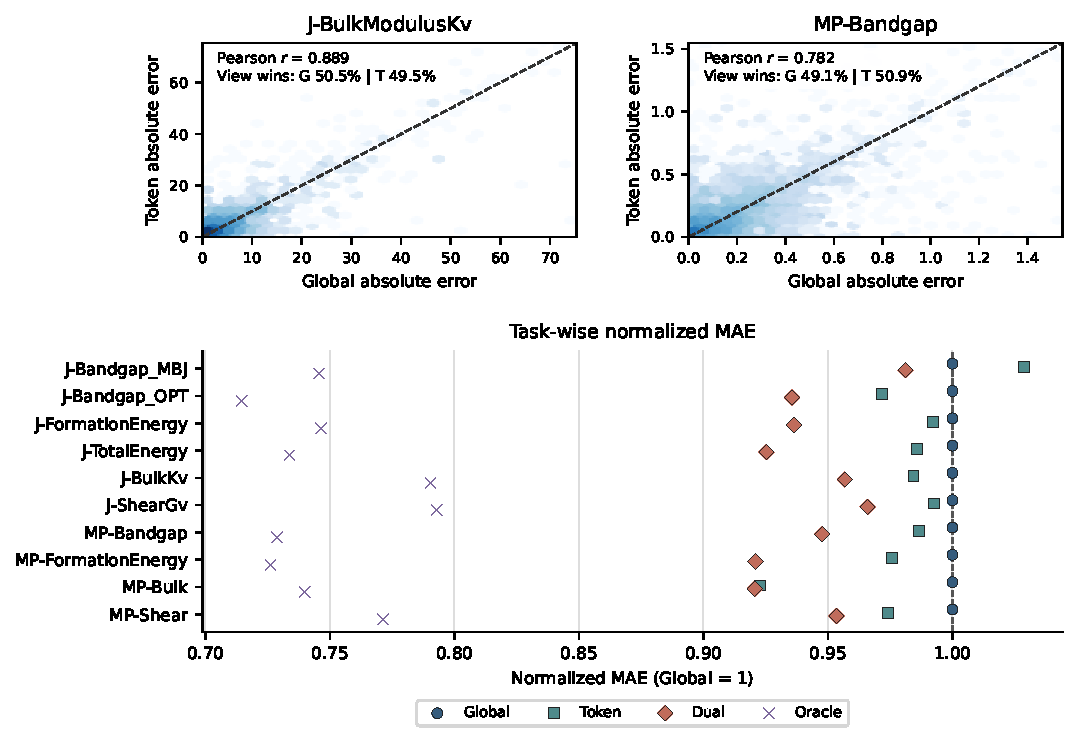
\includegraphics[width=\linewidth]{error_complementarity.pdf}
\caption{Representative sample-level error complementarity analysis from one independent run. Top: hexbin densities for two representative tasks with $y=x$, Pearson $r$, and Global/Token pathway-win ratios (ties excluded). Bottom: grouped dots for Global, Token, fixed prediction-level combination, and diagnostic Oracle MAE across all ten named tasks, normalized by the global pathway. Oracle uses targets and is non-deployable. A representative run is visualized for clarity; quantitative ranges for both runs are reported in Table~\ref{tab:comp}.}\label{fig:comp}\end{figure}

\begin{table}[H]\caption{Run-wise ranges of validation-set complementarity diagnostics across the ten tasks. Win ratios include ties in the denominator.}\label{tab:comp}\centering\small
\begin{tabular}{lcc}\toprule Diagnostic&Run 1 range&Run 2 range\\\midrule
Pearson absolute-error correlation&0.614--0.900&0.591--0.906\\
Oracle gain over global pathway (\%)&20.709--28.546&20.978--28.801\\
Global sample-win ratio (\%)&17.732--48.526&15.147--48.780\\
Token sample-win ratio (\%)&22.565--81.551&16.960--52.316\\
Combined gain over global pathway (\%)&1.886--7.935&2.537--7.971\\\bottomrule
\end{tabular}\end{table}

Across the ten tasks, Pearson absolute-error correlations span 0.614--0.900 in Run 1 and 0.591--0.906 in Run 2. These positive correlations reflect common crystal inputs and graph-encoder architectures, whereas values below one indicate non-identical residual structure. The oracle MAE is 20.709--28.546\% lower than the global pathway in Run 1 and 20.978--28.801\% lower in Run 2. Although oracle selection is not deployable because it uses the target, the persistent gap quantifies available sample-wise complementarity.

The same-view controls therefore provide an important interpretation of the main result: the gain is reproducible at the prediction level, but it should not be attributed uniquely to cross-view representation diversity.

\FloatBarrier
\subsection{Exploratory interaction diagnostics}
To examine whether earlier cross-view interaction is beneficial, we evaluated validation-only latent-level, message-level, and shared-backbone variants. Because their task coverage, reference baselines, and computational budgets are not uniform, these experiments are interpreted as mechanistic probes rather than as a controlled ranking of fusion locations.

Latent interaction through query conditioning, feature refinement, and explicit pairwise coupling produced measurable representation changes, but predictive effects varied across tasks and datasets. Similarly, SEC-SFT text-conditioned message modulation improved several JARVIS tasks while degrading part of the Materials Project mechanical subset; a zero-initialized residual formulation repaired some degradations but did not preserve gains uniformly.

Shared-backbone dual-view fusion retained some sample-wise complementarity: on the balanced six-task subset, the fixed mean improved four tasks and was lower than the better shared branch on five. Taken together, earlier interaction is feasible but remains property dependent under the available validation protocols. Detailed variant-level diagnostics are reported in the Appendix.


\subsection{Computational cost}
The Global and Token predictors contain 2,661,154 and 2,800,739 trainable parameters, respectively, giving 5,461,893 parameters when both independently trained predictors are retained. The fixed prediction mean introduces no additional trainable parameters, although inference requires both graph--text pathways. The Global pathway uses a CLS representation, whereas the Token pathway retains cached contextual token states.

\section{Discussion}
The results answer three linked questions about global and token-level textual information in graph--text crystal property prediction.

First, do document-level CLS and token-level contextual representations contain non-identical predictive information? Their errors are positively correlated but remain below one, with substantial oracle gaps. The fixed prediction-level mean improves all ten test tasks relative to Global in both runs and improves over both constituent predictors on nine of ten tasks in each run. The matched representation ablation further shows that this complementarity is not explained by a universally superior text aggregator, because CLS, masked mean pooling, and cosine attention win different properties under a common head and loss.

Second, is the observed gain purely attributable to cross-view representation complementarity? Same-view controls show that ordinary prediction averaging contributes substantially: both GG and TT reduce error. GT improves over GG but not over TT at the normalized-macro level, so the full gain cannot be attributed uniquely to cross-view diversity.

Third, why retain independent prediction pathways rather than earlier interaction? Validation-only latent-, message-, and shared-backbone diagnostics were property dependent and did not provide uniform improvements. Independent prediction averaging is therefore retained as the principal empirical configuration under the main protocol, without implying a universal ranking of fusion locations.

\section{Limitations}
The current evaluation uses two independent runs, supporting consistency but not formal significance testing; same-view controls also show that ordinary averaging contributes materially. The main Global/Token comparison jointly changes textual abstraction, prediction head, and training objective, while the matched CLS/mean/cosine ablation partially isolates representation choice on one seed and six validation tasks, not as a full two-run replacement.

Published benchmarks use different partitions and target transformations. The two-predictor design increases storage and inference cost, and cache generation, wall-clock time, latency, and peak memory were not benchmarked under one hardware protocol. Robocrystallographer descriptions inherit the scope and heuristics of the generation procedure, and other intermediate text abstractions remain unexplored.

The interaction studies are validation-only, have unequal task coverage, and were not used for test-time model selection. Aggregate attention statistics do not establish chemical causality or sample-level interpretability, and no matched raw-dot-product versus cosine-normalized performance ablation is available; normalization is therefore treated as a numerical control rather than a causal performance claim.

\section{Conclusion}
This study examines complementary document-level and token-level text representations for graph--text crystal property prediction. Two independently trained SFTGNN--MatBERT pathways are combined with a fixed 0.5/0.5 prediction mean. Across ten JARVIS and Materials Project tasks and two training runs, the combined predictor improves over Global on every task, with an average macro relative MAE reduction of approximately $5.9\%$ ($5.875\pm0.036\%$), and outperforms both constituent predictors on nine of ten tasks in each run.

A matched six-task validation ablation shows that CLS, masked mean pooling, and cosine attention are favored by different properties, while same-view ensembles demonstrate that ordinary prediction averaging explains a substantial part of the gain. Earlier latent-, message-, and shared-backbone interactions are likewise property dependent. The principal supported finding is therefore sample-aligned prediction complementarity under the stated protocol, rather than a universally superior textual representation or fusion location.

\appendix
\setcounter{topnumber}{5}
\setcounter{bottomnumber}{5}
\setcounter{totalnumber}{10}
\renewcommand{\topfraction}{0.95}
\renewcommand{\bottomfraction}{0.95}
\renewcommand{\textfraction}{0.05}
\renewcommand{\floatpagefraction}{0.10}
\section{Post-hoc descriptive same-view analysis}
This post-hoc descriptive analysis uses saved test predictions and does not select an architecture or fusion weight. For task $j$, GG and TT average predictions across the two runs, while GT first forms the run-wise Global--Token means. The normalized macro values are Global $=1.000000$, GG $=0.956587$, TT $=0.935789$, and GT $=0.941171$; GT is lower than GG on 9/10 tasks but lower than TT on 3/10. The resulting 5.8829\% versus 5.8754\% reductions differ only because of aggregation order.

\section{Latent interaction diagnostics}\label{app:latent}
These validation-only variants were designed to probe distinct latent interaction mechanisms and were not candidate final models. TAGIF denotes token-anchored global interaction fusion; GCTA denotes CLS-conditioned graph--token attention; GCTR denotes CLS-conditioned token refinement; and PVIN denotes a parallel-view interaction network. Table~\ref{tab:latent_detail} summarizes their representative diagnostics, including cases in which the latent interaction was active but its predictive effect was weak or property dependent.

\begin{table}[!htbp]\caption{Validation-only diagnostics for latent interaction variants. All values are computed on validation sets; no test evaluation is used for these variants.}\label{tab:latent_detail}\centering\scriptsize
\resizebox{\linewidth}{!}{\begin{tabular}{lllll}\toprule
Method&Task&Predictive result&Representation or attention diagnostic&Semantic/control evidence\\\midrule
TAGIF&JARVIS-Bandgap\_MBJ&$-0.975\%$ macro gain vs Token-only over two tasks&innovation ratio 0.989; interaction ratio 0.432&correct CLS control better than shuffled/zero in both tasks\\
TAGIF&MP-Bandgap&0/2 wins vs Token-only&innovation ratio 0.834; interaction ratio 0.695&non-collapsed orthogonal component\\
GCTA&JARVIS-Bandgap\_MBJ&valid MAE 0.285429 vs 0.286644 for naive concat&$||q_c||/||q_g||=0.440$; attention L1 change 0.00218&active $W_{qc}$ gradient\\
GCTA&MP-Bandgap&valid MAE 0.217874 vs 0.219016 for naive concat&$||q_c||/||q_g||=0.194$; attention L1 change 0.00161&active $W_{qc}$ gradient\\
GCTR&JARVIS-Bandgap\_MBJ&degrades by 0.758\% vs naive concat&$\cos(h_t,h_{refined})=0.968$; refinement ratio 0.028&FiLM branch active\\
GCTR&MP-Bandgap&improves by 1.835\% vs naive concat&$\cos(h_t,h_{refined})=0.856$; refinement ratio 0.016&semantic control not consistently effective\\\bottomrule
\end{tabular}}
\end{table}

\section{Message-level interaction diagnostics}\label{app:message}
SEC-SFT introduces text-conditioned modulation into the final SFTConv message construction. The residual formulation adds a zero-initialized text-conditioned correction to the original message. The following tables preserve task-level validation values under the task-specific coverage described in Section~5.5.

\begin{table}[!htbp]
\caption{Message-level validation diagnostics. Panel (a) reports task-wise SEC-SFT relative changes; panel (b) reports the selected residual SEC-SFT comparisons. All values are validation results.}
\label{tab:message_detail}\centering\scriptsize
\textit{(a) SEC-SFT task-wise relative change}\\[-2pt]
\begin{tabular}{lr}\toprule
Task&Relative change (\%)\\\midrule
JARVIS-MBJ&+1.283\\
JARVIS-OPT&+0.660\\
JARVIS-Formation&-1.121\\
JARVIS-Total&+1.740\\
JARVIS-Bulk&+2.418\\
JARVIS-Shear&+2.279\\
MP-Bandgap&+2.206\\
MP-Formation&+1.675\\
MP-Bulk&-3.844\\
MP-Shear&-5.553\\\bottomrule
\end{tabular}
\\[6pt]
\textit{(b) Residual SEC-SFT selected cases}\\[-2pt]
\begin{tabular}{lrrr}\toprule
Task&Original&SEC-SFT&Residual SEC-SFT\\\midrule
MP-Bulk&0.03789499&0.03935185&0.03717689\\
MP-Shear&0.06582852&0.06948390&0.06564737\\
JARVIS-Bulk&9.2148&8.9920&9.3033\\\bottomrule
\end{tabular}
\end{table}

\section{Shared-backbone prediction diagnostics}\label{app:shared}
Shared-backbone dual-view fusion (SBDVF) uses two textual prediction heads with a shared SFTGNN encoder. The following tables report detailed validation diagnostics for the balanced six-task subset.

\begin{table}[!htbp]
\caption{Detailed shared-backbone validation diagnostics for the balanced six-task subset.}
\label{tab:sbdvf_detail}\centering\scriptsize
\begin{tabular}{lrrr}\toprule
Task&Abs.-error corr.&Oracle gain (\%)&Gradient cosine\\\midrule
JARVIS-MBJ&0.941&13.010&+0.477\\
JARVIS-Formation&0.988&9.381&-0.435\\
JARVIS-Bulk&0.987&6.273&+0.956\\
MP-Bandgap&0.929&11.582&+0.476\\
MP-Formation&0.981&10.755&-0.215\\
MP-Shear&0.958&10.140&+0.690\\\bottomrule
\end{tabular}
\end{table}

\begin{table}[!htbp]
\caption{Shared-backbone dual-view validation diagnostics for the balanced six-task subset. Values are MAE; the gain is relative to the matched validation baseline.}
\label{tab:sbdvf_compact}\centering\scriptsize
\begin{tabular}{lrrrrr}\toprule
Task&Original&Shared Global&Shared Token&Final&Gain (\%)\\\midrule
JARVIS-MBJ&0.240074&0.247644&0.244046&0.241591&-0.632\\
JARVIS-Formation&0.028966&0.028823&0.028645&0.028505&+1.591\\
JARVIS-Bulk&9.214838&8.939804&8.887833&8.869501&+3.748\\
MP-Bandgap&0.212996&0.204922&0.202905&0.200832&+5.711\\
MP-Formation&0.020460&0.020200&0.020050&0.019905&+2.712\\
MP-Shear&0.065829&0.066835&0.068522&0.066976&-1.744\\\midrule
Macro gain&&&&&+1.898\\
\bottomrule\end{tabular}
\end{table}


\FloatBarrier
\section*{Acknowledgements}
The authors thank the members of their research group for helpful discussions and acknowledge JARVIS, Materials Project, Robocrystallographer, and MatBERT.
\section*{Funding}
This work was supported by the Industry--University Cooperation Collaborative Education Project of the Ministry of Education (No.~250603873093026), the Fundamental Research Funds for the Central Universities of China (Grant No.~PA2025GDSK0036), and the Innovative Teaching Team for Ideological and Political Education in Electronic Information Science and Technology (No.~2025XKSTD01).
\section*{Data availability}
The source data used in this study are publicly available from JARVIS and Materials Project. Derived descriptions and prediction files supporting the findings will be made available with the final release.
\section*{Code availability}
The model and analysis code will be made available with the final release.
\section*{Declaration of competing interest}
The authors declare no competing interests.
\bibliographystyle{elsarticle-num}
\bibliography{cas-refs}
\end{document}



